\documentclass[12pt]{article}
\title{Dokumentacja implementacji algorytmu wstecznej propagacji na przykładzie funkcji NXoR}
\author{Michał Korniak}
\date{}
\usepackage{graphicx}
\usepackage{graphics}
\usepackage[polish]{babel}
\usepackage[T1]{fontenc}
\newcommand{\source}[1]{{\centerline{\tiny Źródło: #1}}}


\begin{document}
\maketitle
\tableofcontents{}
\newpage


\section{Wprowadzenie}
Algorytm wstecznej propagacji błędu jest metodą uczenia wielowarstwowych polegającą na korekcie wag połączeń między neuronami na podstawie błędu całej sieci.
W tym dokumencie prześledzę działanie tego algorytmu na przykładzie sieci realizującej funkcję NXoR,
jednocześnie przedstawiając jego autorską implementację w języku C\#.

\section{Algorytm wstecznej propagacji}
\subsection{Sposób działania wielowarstwowych sieci neuronowych}
Algorytm wstecznej propagacji jest wykorzystywany do nauczania wielowarstwowych sieci jednokierunkowych.
Taka sieć zawiera warstwę wejściową i warstwę wyjściową,
może posiadać również warstwy ukryte (w zależności od problemu jedną albo dwie).
Każda warstwa zawiera dowolną ilość neuronów.
Neurony są połączone ze sobą w taki sposób, że każdy neuron warstwy innej niż wyjściowa jest połączony z każdym neuronem kolejnej warstwy,
a każde połączenie ma określoną wagę.
Dodatkowo możliwe jest połączenie do tego zwanego biasa, czyli połączenia do neuronu, który zawsze przyjmuje wartość 1.
Połączenia wejściowe do neuronu będą wpływać na to jaką będzie miał wartość.

Rysunek 1 przedstawia przykład jednokierunkowej sieci neuronowej opartej o dwa neurony warstwy wejściowej i tyle samo neuronów w warstwach ukrytej i wyjściowej. 
Oprócz połączeń do innych neuronów, istnieją również połączenia do biasa, który jest wspólny dla neuronów w ramach jednej warstwy.

\begin{figure}[!ht]
    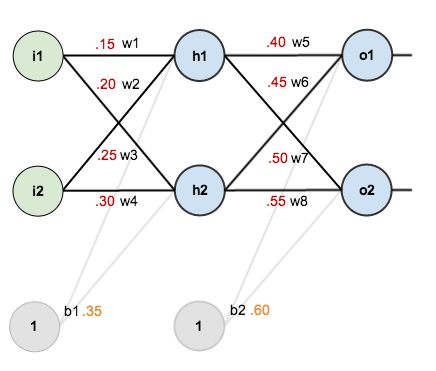
\includegraphics[width=\linewidth]{images/feed-forward-diagram.png}
    \source{https://mattmazur.com/2015/03/17/a-step-by-step-backpropagation-example/}
    \caption{Przykład wielowarstwowej sieci jednokierunkowej}
\end{figure}

Rysunek 1 zawiera wartości neuronów wejściowych oraz wag, dzięki czemu będziemy mogli pokazać jak wyliczane są wartości kolejnych neuronów.
Robimy to sumując wartości połączeń do tego wektora, a następnie poddając wynik funkcji aktywacji.
Przez wartość połączenia będziemy rozumieli iloczyn wagi i neuronu wejściowego dla połączenia.
Przykładowo dla neuronu h1 wartość przed użyciem funkcji aktywacji będzie równa:
\[
  net = i1*w1+i2*w2+1*b1
\]
Co po podstawieniu wartości da:
\[
  net_{h1} = 0.05*0.15+0.10*0.20+1*0.35=0.3775
\]
Taka wartość jest następnie poddawana działaniu funkcji aktywacji. 
Takie działanie umożliwia normalizowanie wartości neuronów do oczekiwanych przedziałów wartości.
W tym przypadku skorzystamy z funkcji sigmoidalnej, której zakres wartości mieści się w przedziale [0,1]:
\[
    f(x) =  \frac{\mathrm{1} }{\mathrm{1} + e^{-x} } 
\]
Po podstawieniu otrzymanej wcześniej wartości do funkcji dostaniemy wartość neuronu h1:
\[
    out_{h1} 
    = f(net_{h1}) 
    =  \frac{\mathrm{1} }{\mathrm{1} + e^{-net_{h1}} } 
    =  \frac{\mathrm{1} }{\mathrm{1} + e^{-0.3775} } \approx 0.5932
\]
W ten sposób będziemy liczyć wartość kolejnych neuronów aż otrzymamy wynik.

\subsection{Implementacja wielowarstwowej sieci neuronowej}





\end{document}

